\documentclass{beamer}

\usepackage{algorithm}
\usepackage{algpseudocode}

\usefonttheme{serif}
\usepackage{dsfont}
\setbeamersize{text margin left=5pt, text margin right=5pt}

\newcommand{\bgk}[1]{\boldsymbol{#1}}

\newcommand{\bzero}{\bgk{0}}
\newcommand{\bone}{\bgk{1}}

\newcommand{\balpha}{\bgk{\alpha}}
\newcommand{\bnu}{\bgk{\nu}}
\newcommand{\bbeta}{\bgk{\beta}}
\newcommand{\bxi}{\bgk{\xi}}
\newcommand{\bgamma}{\bgk{\gamma}} 
\newcommand{\bo}{\bgk{o }}
\newcommand{\bdelta}{\bgk{\delta}}
\newcommand{\bpi}{\bgk{\pi}}
\newcommand{\bepsilon}{\bgk{\epsilon}} 
\newcommand{\bvarepsilon}{\bgk{\varepsilon}} 
\newcommand{\brho}{\bgk{\rho}}
\newcommand{\bvarrho}{\bgk{\varrho}}
\newcommand{\bzeta}{\bgk{\zeta}}
\newcommand{\bsigma}{\bgk{\sigma}}
\newcommand{\boldeta}{\bgk{\eta}}
\newcommand{\btay}{\bgk{\tau}}
\newcommand{\btheta}{\bgk{\theta}}
\newcommand{\bvertheta}{\bgk{\vartheta}}
\newcommand{\bupsilon}{\bgk{\upsilon}}
\newcommand{\biota}{\bgk{\iota}}
\newcommand{\bphi}{\bgk{\phi}}
\newcommand{\bvarphi}{\bgk{\varphi}}
\newcommand{\bkappa}{\bgk{\kappa}}
\newcommand{\bchi}{\bgk{\chi}}
\newcommand{\blambda}{\bgk{\lambda}}
\newcommand{\bpsi}{\bgk{\psi}}
\newcommand{\bmu}{\bgk{\mu}}
\newcommand{\bomega}{\bgk{\omega}}

\newcommand{\bA}{\bgk{A}}
\newcommand{\bDelta}{\bgk{\Delta}}
\newcommand{\bLambda}{\bgk{\Lambda}}
\newcommand{\bSigma}{\bgk{\Sigma}}
\newcommand{\bOmega}{\bgk{\Omega}}

\newcommand{\bvec}[1]{\mathbf{#1}}

\newcommand{\va}{\bvec{a}}
\newcommand{\vb}{\bvec{b}}
\newcommand{\vc}{\bvec{c}}
\newcommand{\vd}{\bvec{d}}
\newcommand{\ve}{\bvec{e}}
\newcommand{\vf}{\bvec{f}}
\newcommand{\vg}{\bvec{g}}
\newcommand{\vh}{\bvec{h}}
\newcommand{\vi}{\bvec{i}}
\newcommand{\vj}{\bvec{j}}
\newcommand{\vk}{\bvec{k}}
\newcommand{\vl}{\bvec{l}}
\newcommand{\vm}{\bvec{m}}
\newcommand{\vn}{\bvec{n}}
\newcommand{\vo}{\bvec{o}}
\newcommand{\vp}{\bvec{p}}
\newcommand{\vq}{\bvec{q}}
\newcommand{\vr}{\bvec{r}}
\newcommand{\vs}{\bvec{s}}
\newcommand{\vt}{\bvec{t}}
\newcommand{\vu}{\bvec{u}}
\newcommand{\vv}{\bvec{v}}
\newcommand{\vw}{\bvec{w}}
\newcommand{\vx}{\bvec{x}}
\newcommand{\vy}{\bvec{y}}
\newcommand{\vz}{\bvec{z}}

\newcommand{\vA}{\bvec{A}}
\newcommand{\vB}{\bvec{B}}
\newcommand{\vC}{\bvec{C}}
\newcommand{\vD}{\bvec{D}}
\newcommand{\vE}{\bvec{E}}
\newcommand{\vF}{\bvec{F}}
\newcommand{\vG}{\bvec{G}}
\newcommand{\vH}{\bvec{H}}
\newcommand{\vI}{\bvec{I}}
\newcommand{\vJ}{\bvec{J}}
\newcommand{\vK}{\bvec{K}}
\newcommand{\vL}{\bvec{L}}
\newcommand{\vM}{\bvec{M}}
\newcommand{\vN}{\bvec{N}}
\newcommand{\vO}{\bvec{O}}
\newcommand{\vP}{\bvec{P}}
\newcommand{\vQ}{\bvec{Q}}
\newcommand{\vR}{\bvec{R}}
\newcommand{\vS}{\bvec{S}}
\newcommand{\vT}{\bvec{T}}
\newcommand{\vU}{\bvec{U}}
\newcommand{\vV}{\bvec{V}}
\newcommand{\vW}{\bvec{W}}
\newcommand{\vX}{\bvec{X}}
\newcommand{\vY}{\bvec{Y}}
\newcommand{\vZ}{\bvec{Z}}

\usepackage{subcaption}
\newcommand{\bitem}{\item[$\bullet$]}

\usepackage{xcolor}
\usepackage[utf8]{inputenc}
\DeclareFontEncoding{LS1}{}{}
\DeclareFontSubstitution{LS1}{stix}{m}{n}
\DeclareSymbolFont{symbols2}{LS1}{stixfrak} {m} {n}
\DeclareMathSymbol{\operp}{\mathbin}{symbols2}{"A8}
\setbeamertemplate{navigation symbols}{}

\usepackage{lipsum}

\newcommand\blfootnote[1]{%
  \begingroup
  \renewcommand\thefootnote{}\footnote{#1}%
  \addtocounter{footnote}{-1}%
  \endgroup
}

\addtobeamertemplate{navigation symbols}{}{%
    \usebeamerfont{footline}%
    \usebeamercolor[fg]{footline}%
    \hspace{1em}%
    \insertframenumber/\inserttotalframenumber
}

\title{
Trace Estimation III\\
-- Making the most of every sample -- \\
Lecture 7
}
%\subtitle{Mathematical framework, existence and exactness}

\author{F. M. Faulstich}
\date{01/30/2024}


\begin{document}

\frame{\titlepage}


\begin{frame}{Implicit Trace Estimation Problem}

\begin{itemize}
    \bitem Given access to $\vA\in\mathbb{F}^{n \times n}$ via the MatVec product $\vx \mapsto \vA\vx$, estimate its trace:
$$
{\rm Tr}(\vA)
=
\sum_{i= i}^n (\vA)_{ii}
$$
\pause
\bitem [Girard--Hutchinson estimator] Let $\{\bomega_i\}$ be isotropic and i.i.d.~then
$$
\hat{\rm tr}_{\rm GH}
:=
\frac{1}{m}
\sum_{i=1}^m
\bomega_i^* (A\bomega_i)
$$
is an unbiased estimator of the trace
$$
\mathbb{E}(\hat{\rm tr}_{\rm GH})
=
{\rm Tr}(\vA).
$$
\bitem We found
$$
\mathbb{V} (\hat{\rm tr}_{\rm GH})
=
\frac{1}{m}
\mathbb{V}(\bomega^* (A\bomega))
\in \mathcal{O}\left(\frac{1}{m}\right)
$$
$\Rightarrow$ Converges as $\mathcal{O}\left(\frac{1}{\sqrt{m}}\right)$
(Monte-Carlo)
\end{itemize}

\end{frame}


\begin{frame}{Variance reduction (H\small{UTCH\texttt{++}})}

Given $m$ -- a fixed number of MatVecs:
\begin{itemize}
    \bitem Sample isotropic i.i.d.~$\bomega_1,...,\bomega_{2m/3}$ 
    \bitem Sketch $\vY = \vA[\bomega_{m/3 + 1}|\bomega_{m/3 + 2}|...|\bomega_{2m/3}]$
    \bitem Orthonormalize $\vQ = {\rm orth}(\vY)$
    \bitem Output estimator
    $$
    \hat{\rm tr}_{H++}
    =
    {\rm Tr}(\vQ^* (\vA \vQ))
    +
    \frac{1}{m/3} 
    \sum_{i=1}^{m/3}
    \bomega_i^* (\vI - \vQ \vQ^*)
    \big(\vA (\vI - \vQ \vQ^*) \bomega_i\big)
    $$
\end{itemize}
\end{frame}

\begin{frame}{}
    \begin{itemize}
        \bitem Recall that $\hat \vA = \vQ \vQ^* \vA$ is a low rank approximation of $\vA$
        \bitem H{\footnotesize UTCH\texttt{++}} computes the trace of this low-rank approximation
        $$
        {\rm Tr}(\hat \vA)
        =
        {\rm Tr}(\vQ \vQ^* \vA)
        =
        {\rm Tr}(\vQ^* (\vA\vQ))
        $$
        and then applies the Girard--Hutchinson estimator to the residual
        $$
        {\rm Tr}(\vA - \hat{\vA})
        =
        {\rm Tr}((\vI - \vQ \vQ^*)\vA)
        =
        {\rm Tr}((\vI - \vQ \vQ^*)\vA(\vI - \vQ \vQ^*))
        $$
        \bitem H{\footnotesize UTCH\texttt{++}} is an unbiased trace estimator of $\vA$
        $$
        \mathbb{E}(\hat{\rm tr}_{{\rm H}++})
        =
        {\rm Tr}(\vA)
        $$
        and 
        $$
        \mathbb{V}(\hat{\rm tr}_{{\rm H}++})\in \mathcal{O}\left(
        \frac{1}{m^2}
        \right)
        $$
    \end{itemize}
\end{frame}



\begin{frame}{H\small{UTCH\texttt{++}} Pseudocode}

\begin{itemize}
    \bitem Input: $\vA\in\mathbb{F}^{n\times n}$, $m$ with ${\rm mod}(m,3) = 0$ 
    \bitem Output: $\hat{\rm tr}_{{\rm H}++}$
    \bitem Draw iid isotropic $\bomega_1,...,\bomega_{2m/3}\in\mathbb{F}^n$
    \bitem $\vY = \textcolor{red}{\vA[\bomega_{m/3 + 1}|\bomega_{m/3 + 2}|...|\bomega_{2m/3}]}$
    \bitem $\vQ = {\rm orth}(\vY)$
    \bitem $\vG = [\bomega_{1}|\bomega_{2}|...|\bomega_{m/3}] - \vQ \vQ^*[\bomega_{1}|\bomega_{2}|...|\bomega_{m/3}] $
    \bitem $\hat{\rm tr}_{{\rm H}++} = {\rm Tr}(\vQ^* (\textcolor{red}{\vA \vQ}))
 - \frac{1}{m/3} {\rm Tr}(\vG^* (\textcolor{red}{\vA \vG}))$
\end{itemize}

Indeed, we require $m$ MatVecs
\end{frame}

\begin{frame}{Exchangeable}

\begin{itemize}
    \bitem Exchangeability principle:\\
    If the test vectors $\bomega_1,...,\bomega_k$ are exchangeable, the ``minimum-variance estimator'' is always a symmetric function or $\bomega_1,...,\bomega_k$\\
    $[$invariant under application of the symmetric group ($\bomega_{\sigma(1)},...,\bomega_{\sigma(k)}$)$]$
    \bitem An estimator is exchangeable, if it is invariant under under application of the symmetric group
    \bitem Exchangeability can be seen as a ``robustness'' property of probabilistic algorithms:\\
    \begin{center}
    ``Exchangeability implies that each element in the sequence of estimators contributes equally to the estimation'' process
    \end{center}
    \pause 
    \bitem The H{\footnotesize UTCH\texttt{++}} estimator is not exchangeable\\
    $[$it uses some test vectors to perform low-rank approx$]$
\end{itemize}
\begin{center}
    $\Rightarrow$ Development of XT{\footnotesize RACE} estimator
\end{center}
\end{frame}

\begin{frame}{XT{\small RACE} Estimator}

\only<1>{Idea: Use all but one test vector to form a low-rank approximation, and only use the remaining test vector to estimate the trace of the residual.}
\only<2>{
\begin{itemize}
    \bitem Draw $\bomega_1,...,\bomega_{m/2}$ i.i.d.~isotropic test vectors, and form
    $$
    \bOmega := [\bomega_1|...|\bomega_{m/2}]
    $$
    \bitem Construct the orthonormal matrices
    $$
    \vQ_{(i)} = {\rm orth} (A \bOmega_{-i})
    $$
    where $\bOmega_{-i}$ is the test matrix with the i$th$ column removed.
    \bitem Compute the basic estimators
    $$
    \hat{\rm tr}_i
    :=
    {\rm Tr} (\vQ_{(i)}^* (\vA \vQ_{(i)}))
    +
    \bomega_i^* 
    (\vI - \vQ_{(i)}\vQ_{(i)}^*) 
    (\vA (\vI - \vQ_{(i)}\vQ_{(i)}^*) \bomega_i )
    $$
    \bitem m/2. The X{\footnotesize TRCE} estimator averages these basic estimators:
    $$
    \hat{\rm tr}_X
    :=
    \frac{1}{m/2}
    \sum_{i=1}^{m/2}
    \hat{\rm tr}_i
    $$
\end{itemize}
}
\only<3>{
\begin{itemize}
    \bitem The X{\footnotesize TRCE} estimator is an unbiased estimator of ${\rm Tr}(\vA)$
    \bitem The X{\footnotesize TRCE} estimator is invariant under the action of the symmetry group
\end{itemize}
}
\end{frame}

\begin{frame}{XT{\small RACE} Estimator Na\"ive Implementation}

\begin{itemize}
    \bitem Input: $\vA\in\mathbb{F}^{n \times n}$, $m$ with ${\rm mod}(m,2) = 0$
    \bitem Output: $\hat{\rm tr}_X$ and trace error estimate
    \bitem Draw i.i.d~isotropic $\bomega_1,...,\bomega_{m/2}$
    \bitem $\vY = \textcolor{red}{\vA [\bomega_1|...|\bomega_{m/2}]}$
    \bitem for i=1 to m/2\\
    $\qquad \vQ_{(i)} = {\rm ortho}(\vY_{-i})$\\
    $\qquad \hat{\rm tr_i} = {\rm Tr} (\vQ_{(i)}^* (\textcolor{red}{\vA \vQ_{(i)}}))
    +
    \bomega_i^* 
    (\vI - \vQ_{(i)}\vQ_{(i)}^*) 
    (\textcolor{red}{\vA (\vI - \vQ_{(i)}\vQ_{(i)}^*) \bomega_i} )$
    \bitem $\hat{\rm tr} = \frac{1}{m/2} \sum_{i=1}^{m/2} \hat{\rm tr_i}$
    \bitem $\hat{\rm err} ^2 = \frac{1}{(m/2)(m/2-1)} \sum{i=1}^{m/2} (\hat{\rm tr_i} - \hat{\rm tr})^2$
\end{itemize}
\end{frame}

\begin{frame}{XN{\small YS}T{\small RACE} Estimator}

\begin{itemize}
    \bitem The central idea of the variance improved estimators is to use a low-rank approximation of $\vA$
    \bitem For an arbitrary matrix this requires 
    \bitem What about $\vA \in \mathbb{H}_n$ and $0\preccurlyeq\vA $?
\end{itemize}
\begin{center}
     $\Rightarrow$ Nystr\"om approximation
\end{center}
\end{frame}

\begin{frame}{Nystr\"om approximation}
\begin{itemize}
    \bitem Let $\vA \in \mathbb{H}_n$ and $0\preccurlyeq\vA $. Then 
    $$
    \vA \langle \vX \rangle
    =
    \vA\vX (\vX^* \vA \vX)^{\dagger} (\vA \vX)^*
    =
    \vY (\vX^* \vY)^{\dagger} \vY^*
    $$
    is the Nystr\"om approximation for a test matrix $\vX \in \mathbb{F}^{n\times s}$.
    \bitem Clearly ${\rm rank}(\vA \langle \vX \rangle) \leq s$.
    \bitem Note that we only need a single application of $\vA \vX$ to compute the Nystr\"om approximation.
    \bitem The randomized SVD requires two!
\end{itemize}

\begin{center}
    $\Rightarrow$ The Nystr\"om approximation only requires $k$ MatVecs whereas the randomized SVD requires $2k$ MatVecs.
\end{center}

\end{frame}


\begin{frame}{Why does it work?}
Proof for block matrix formulation
\begin{itemize}
    \bitem Recall for 
    $$
    \vA = 
    \begin{pmatrix}
    \vW & \vB^T\\
    \vB & \vC
    \end{pmatrix}
    $$
    we have $\vA/\vW = \vC - \vB \vW^{-1} \vB^T$
    \bitem The Nystr\"om approximation is given by
    $$
    \tilde{\vA}
    =
    \begin{pmatrix}
    \vW\\ \vB
    \end{pmatrix}
    \vW^{-1}
     \begin{pmatrix}
    \vW & \vB^T
    \end{pmatrix}
    =
    \begin{pmatrix}
    \vW & \vB^T\\
    \vB & \vB \vW^{-1}\vB^T
    \end{pmatrix}
    $$
    \bitem Let's look at 
    $$
    \vA - \tilde{\vA}
    =
    \begin{pmatrix}
    \vW & \vB^T\\
    \vB & \vC
    \end{pmatrix}
    -
    \begin{pmatrix}
    \vW & \vB^T\\
    \vB & \vB \vW^{-1}\vB^T
    \end{pmatrix}
    =
    \begin{pmatrix}
    \bzero & \bzero\\
    \bzero & \vA/\vW
    \end{pmatrix}
    $$
    \bitem Note: Nystr\"om is a rough approximation
\end{itemize}
    
\end{frame}

\begin{frame}{XN{\small YS}T{\small RACE} Estimator Na\"ive}

\begin{itemize}
    \bitem Input: $\vA \in \mathbb{H}_n$ with $0\preccurlyeq\vA $, and $m\in\mathbb{N}$
    \bitem Output: $\hat{tr}_{\rm XN}$, and trace error estimate
    \bitem Draw i.i.d.~isotropic $\bomega_1,...,\bomega_m$
    \bitem $\bOmega = [\bomega_1|...|\bomega_m]$
    \bitem $\vY = \vA \bOmega$
    \bitem for i = 1 to m\\
    $\qquad \vA_i = \vY_{-i} (\bOmega_{-i}^* \vY_{-i})^\dagger \vY^*_{-i}$\\
    $\qquad \hat{\rm tr}_i = {\rm Tr}(\vA_i) + \bomega_i^*((A - A_i)\bomega_i)$\\
    $\hat{\rm tr}_{\rm XN} = \frac{1}{m} \sum_{i=1}^m \hat{\rm tr}_i$\\
    $\hat{\rm err}^2 = \frac{1}{m(m-1)} \sum_{i=1}^m (\hat{\rm tr} _i - \hat{\rm tr} )^2$
\end{itemize}
\end{frame}

\begin{frame}{Computational Performance}

Set up:
\begin{itemize}
    \bitem Consider the matrix $$
    \vA (\blambda) = \vU {\rm diag}(\blambda) \vU^*
    $$ 
    where $\vU$ is a Haar random orthogonal matrix.
    \bitem A Haar random orthogonal matrix is a matrix drawn uniformly from the set of all orthogonal matrices of a given size:\\
    \begin{itemize}
        \item[i)] Generate a $\vA \sim \mathcal{N}(\bzero, \vI)$
        \item[ii)] $[\vQ,\vR] = {\rm qr}(\vA)$
        \item[iii)] $\vD = {\rm diag}({\rm sign}({\rm diag}(R)))$
        \item[iv)] $\vQ = \vQ  \vD$
    \end{itemize}
    \bitem For $\blambda$ four choices are considered:
    \begin{itemize}
        \item[i)] flat: $\blambda = (3-2(i-1)/(N-1)~:~ i = 1,2,...,N)$ 
        \item[ii)] poly: $\blambda = (i^{-2}~:~ i = 1,2,...,N)$
        \item[iii)] \underline{exp}: $\blambda = (0.7^i~:~ i = 0,2,...,N-1)$
        \item[iv)] step: 
        $\blambda = (\underbrace{1,...,1}_{50{\rm~times}}, \underbrace{10^{-3},...,10^{-3}}_{N-50{\rm~times}})$
    \end{itemize}
\end{itemize}
\end{frame}

\begin{frame}{Computational Performance}

\begin{itemize}
    \bitem Apply the estimators to a random PSD matrix with exponentially decreasing eigenvalue
    \bitem Run 1000 trails for feasible $m$
    \bitem compute the averaged error of the trace per estimator
\end{itemize}

\begin{figure}
    \centering
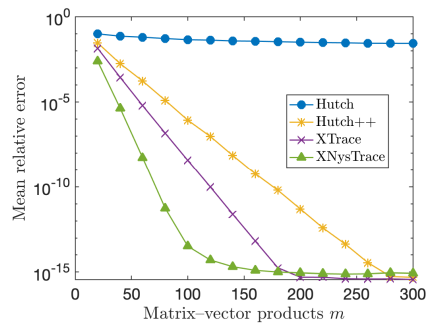
\includegraphics[width = 0.5\textwidth]{Graphics/TraceEstimators.png}
\caption{Computational performance of different trace estimators\footnote{Epperly, Tropp, Webber, SIMAX, 2024}}
\end{figure}


    
\end{frame}
\end{document}




